\chapter{Application Development}

\section{System Architecture}
\begin{figure}[H]\centering
\begin{tikzpicture}[x=1cm,y=1cm, box/.style={draw, rounded corners=2pt, align=center, font=\sffamily\footnotesize, inner sep=4pt, fill=#1}, box/.default=white, arr/.style={-{Stealth[length=2mm]}, line width=0.6pt}]
  \node[box=blue!6, text width=3.3cm] (ui) at (-0.2,0) {\textbf{Browser}\\React 18 single-page app\\(one workspace per role)};
  \node[box=orange!8, text width=4.9cm] (api) at (6.6,0) {\textbf{API server} (Node.js, Express)\\JWT check $\to$ role check (\texttt{authorize})\\$\to$ controller $\to$ service\\transaction + audit row (\texttt{withTransaction})};
  \node[box=green!8, text width=3.2cm] (db) at (13.4,0) {\textbf{MySQL 9.7.1}\\\texttt{hospital\_db} (InnoDB)\\tables, views, triggers};
  \draw[arr] ([yshift=3pt]ui.east) -- node[above, font=\sffamily\tiny, align=center] {HTTPS, JSON\\(Axios)} ([yshift=3pt]api.west);
  \draw[arr] ([yshift=-3pt]api.west) -- node[below, font=\sffamily\tiny, align=center] {Socket.IO\\events} ([yshift=-3pt]ui.east);
  \draw[arr] ([yshift=3pt]api.east) -- node[above, font=\sffamily\tiny, align=center] {SQL\\(mysql2 pool)} ([yshift=3pt]db.west);
  \draw[arr] ([yshift=-3pt]db.west) -- node[below, font=\sffamily\tiny] {rows} ([yshift=-3pt]api.east);
  \node[font=\sffamily\tiny, align=center] at (13.4,-1.45) {restricted account \texttt{hospital\_app}\\(SELECT, INSERT, UPDATE, DELETE, EXECUTE)};
\end{tikzpicture}
\caption{Architecture: three tiers; the database is reached only through the API's restricted account}\label{fig:arch}
\end{figure}

\section{Front-End Technologies}
JavaScript throughout. The client is React 18 with React Router 6 (role-guarded routes), built with Vite 4, calling
the API through Axios and receiving live updates (bed changes, the doctor's queue, the emergency queue) over the
Socket.IO client. The API is Express 4 on Node.js with \texttt{mysql2/promise}, \texttt{jsonwebtoken} (sign-in
tokens), \texttt{bcryptjs} (password hashes) and Multer (lab report uploads). Tests use \texttt{node:test} and Puppeteer.

\section{Application Modules}
The API has 24 routers under \texttt{/api}. They map to the ER modules:
\begin{itemize}
\item \textbf{Patients and visits:} registration and search, appointments, the visit state machine (arrive, triage, start, finish), vital signs, consultation notes.
\item \textbf{Clinical orders:} prescriptions with structured dosing, surgery requests; the nurse's MAR (doses due, given, refused, missed).
\item \textbf{Pharmacy:} the dispense queue, dispensing by batch, stock receipt and adjustment, low-stock and expiry views.
\item \textbf{Laboratory:} the order board, results with automatic flagging, report uploads and secure downloads.
\item \textbf{Beds and admissions:} the bed board, admission and discharge, emergency queue and allocation, ambulances, billing.
\item \textbf{Staff and audit:} staff accounts, nurse ward assignments, doctor dashboard statistics, the audit log viewer.
\end{itemize}

\section{Database Connectivity}
\begin{itemize}
\item \textbf{Pool:} \texttt{server/config/db.js} creates a \texttt{mysql2} connection pool (20 connections) from
\texttt{server/.env}. All SQL uses placeholders (\texttt{?}), so user input is never spliced into a statement.
\item \textbf{Time:} every connection stores and reads date-times in UTC (\texttt{SET time\_zone = '+00:00'}),
whatever the time zone of the MySQL server or the API process. ``Today'' (today's appointments, ages, expiry, who is
on a ward) is the date in India, decided by the API (\texttt{server/utils/clock.js}) and passed to SQL as a
parameter, never \texttt{CURDATE()}.
\item \textbf{Restricted account:} the running API connects as \texttt{hospital\_app}, which can read and write rows
and call procedures but cannot change the schema; migrations use a separate administrative account.
\item \textbf{Transactions:} \texttt{withTransaction(req, fn)} takes a connection, begins a transaction, runs the
change and its audit row on that connection, then commits (or rolls back on any error) and releases it.
\item \textbf{Access control:} every route checks the token and the role (\texttt{authorize}); patient data is
further limited to a doctor's care set or a nurse's assigned wards (\texttt{utils/patientAccess.js}).
\end{itemize}

\section{Application Screenshots}
The screenshots (Figure~\ref{fig:screens} and Appendix~C) were taken from the application running on the test
database, which holds only made-up people.

\begin{figure}[H]\centering
\begin{tabular}{@{}cc@{}}
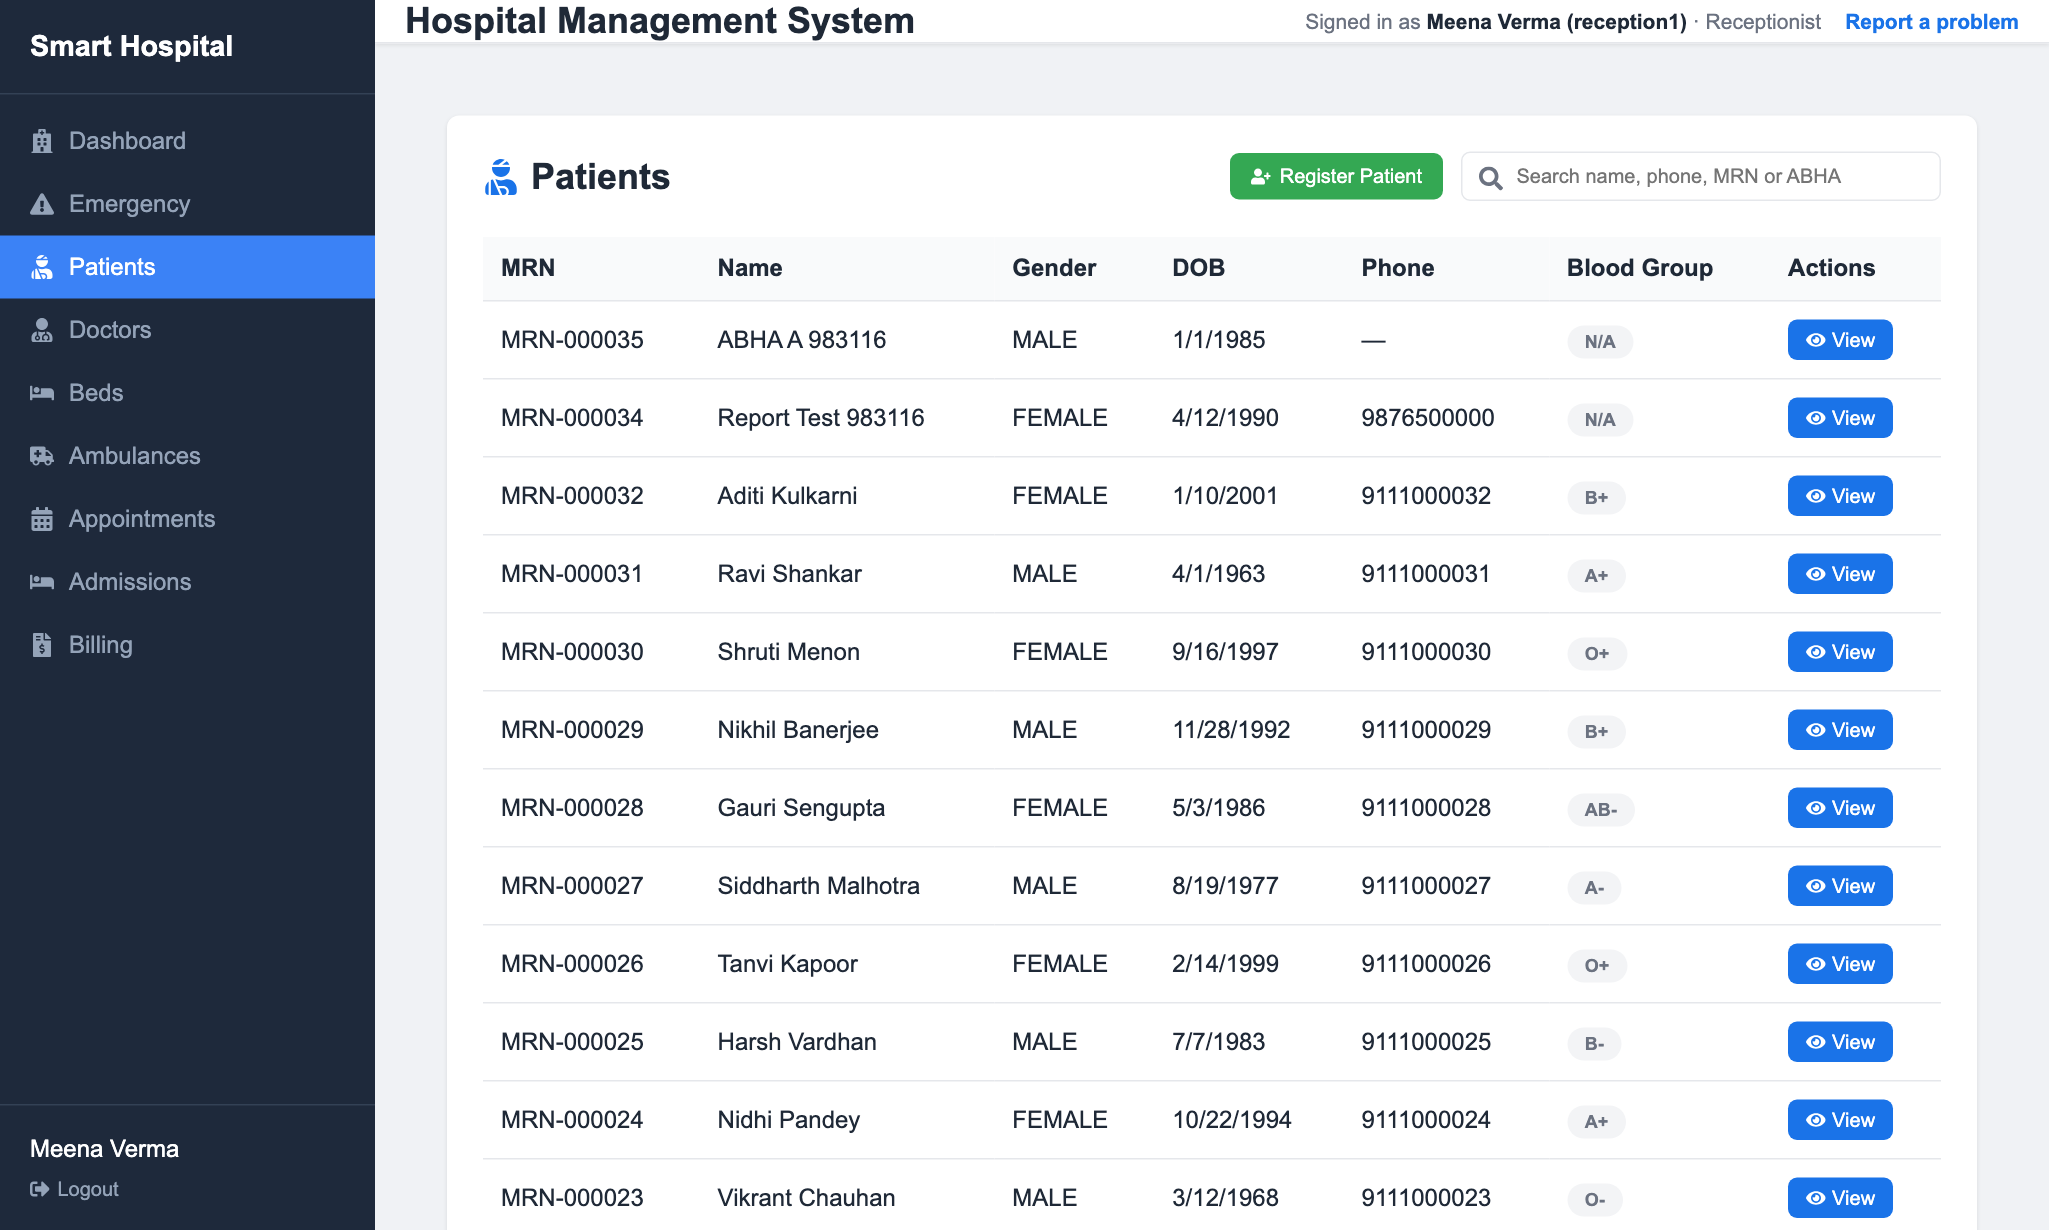
\includegraphics[width=0.485\textwidth]{reception-patients.png} & 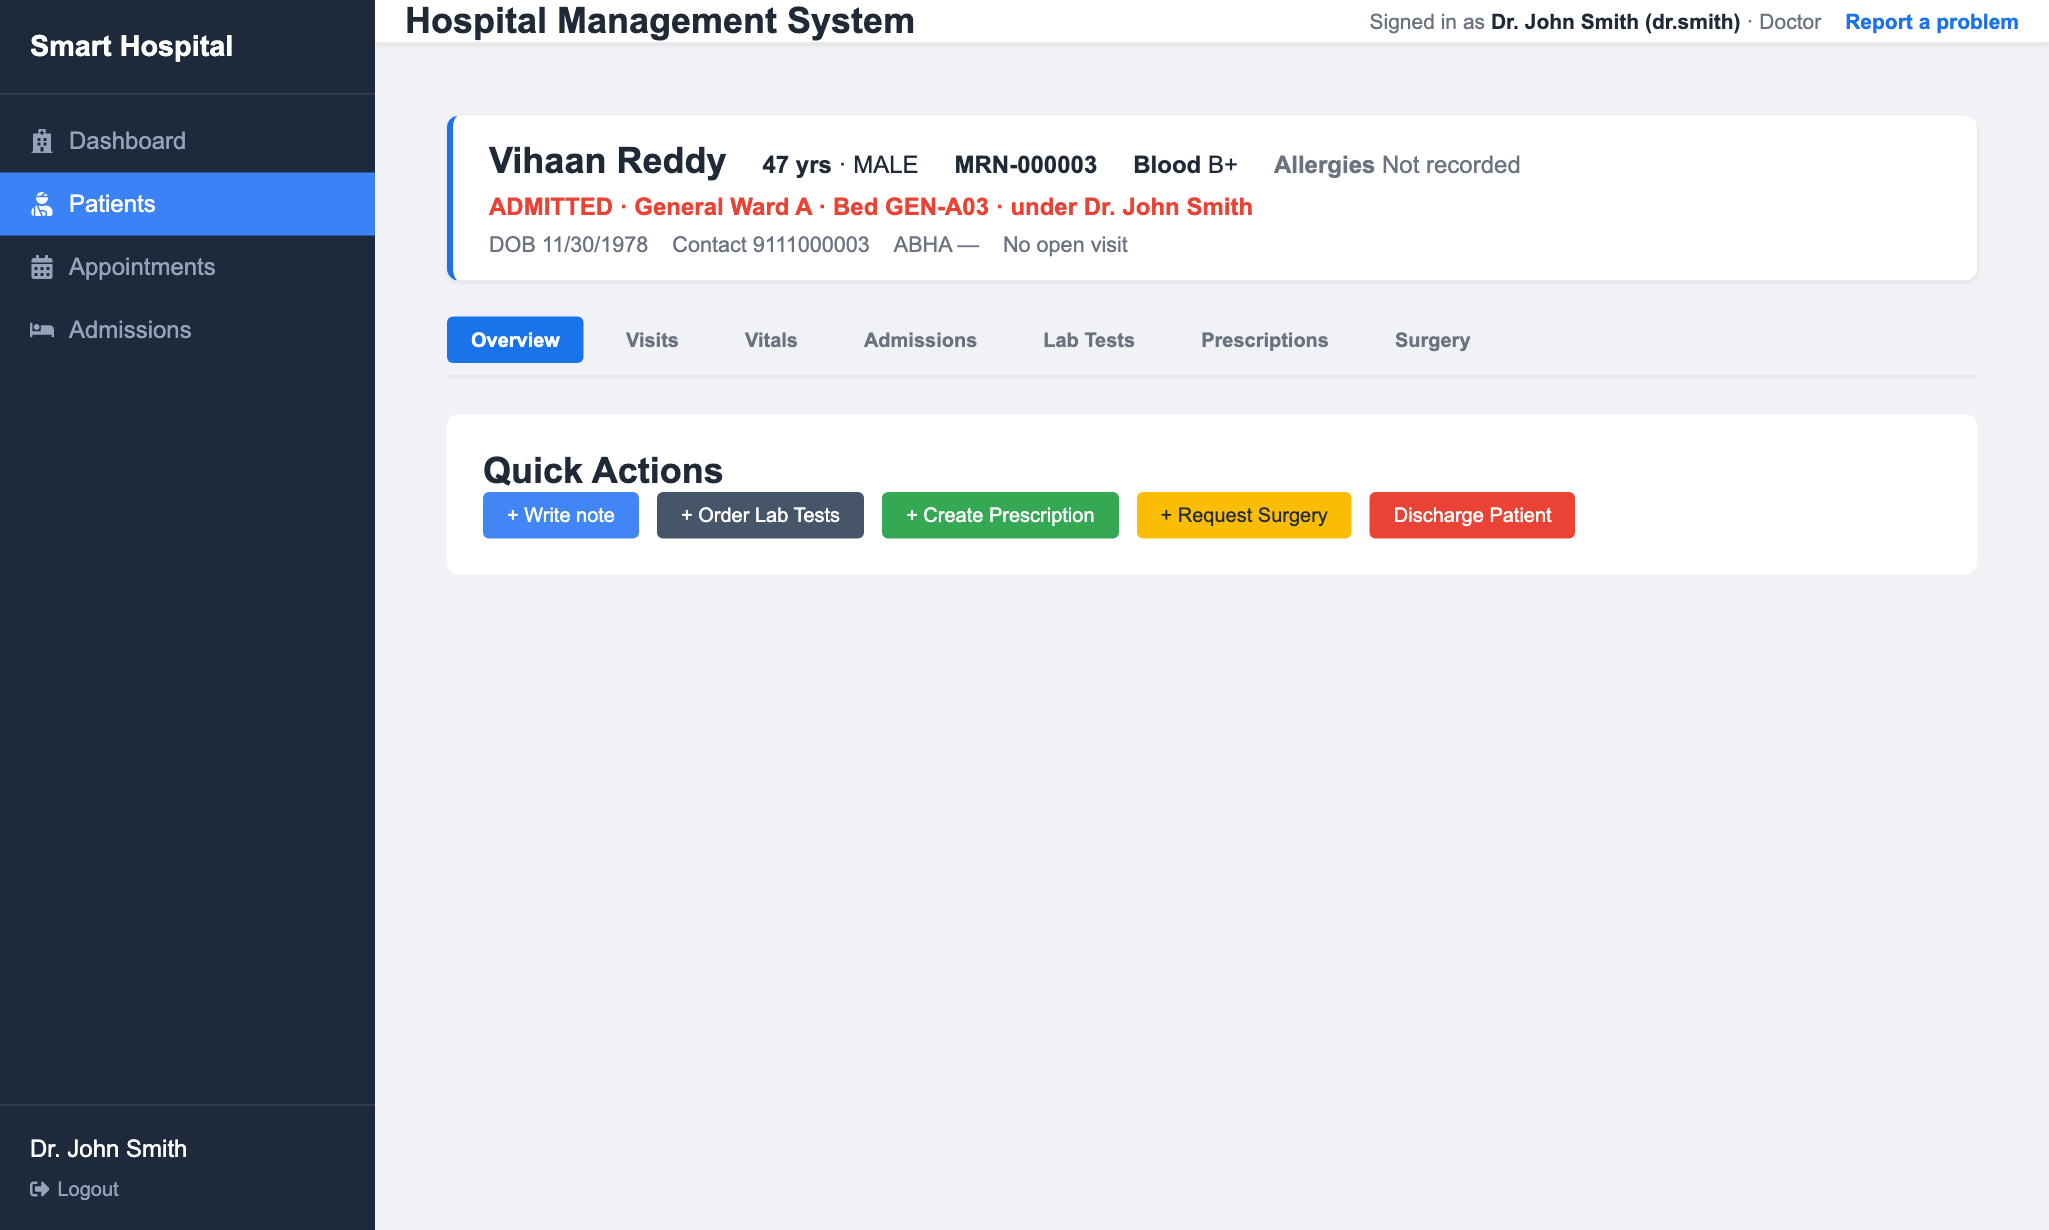
\includegraphics[width=0.485\textwidth]{doctor-patient.png} \\
\small (a) Receptionist: patient list and search & \small (b) Doctor: a patient's visits, notes and orders \\[3pt]
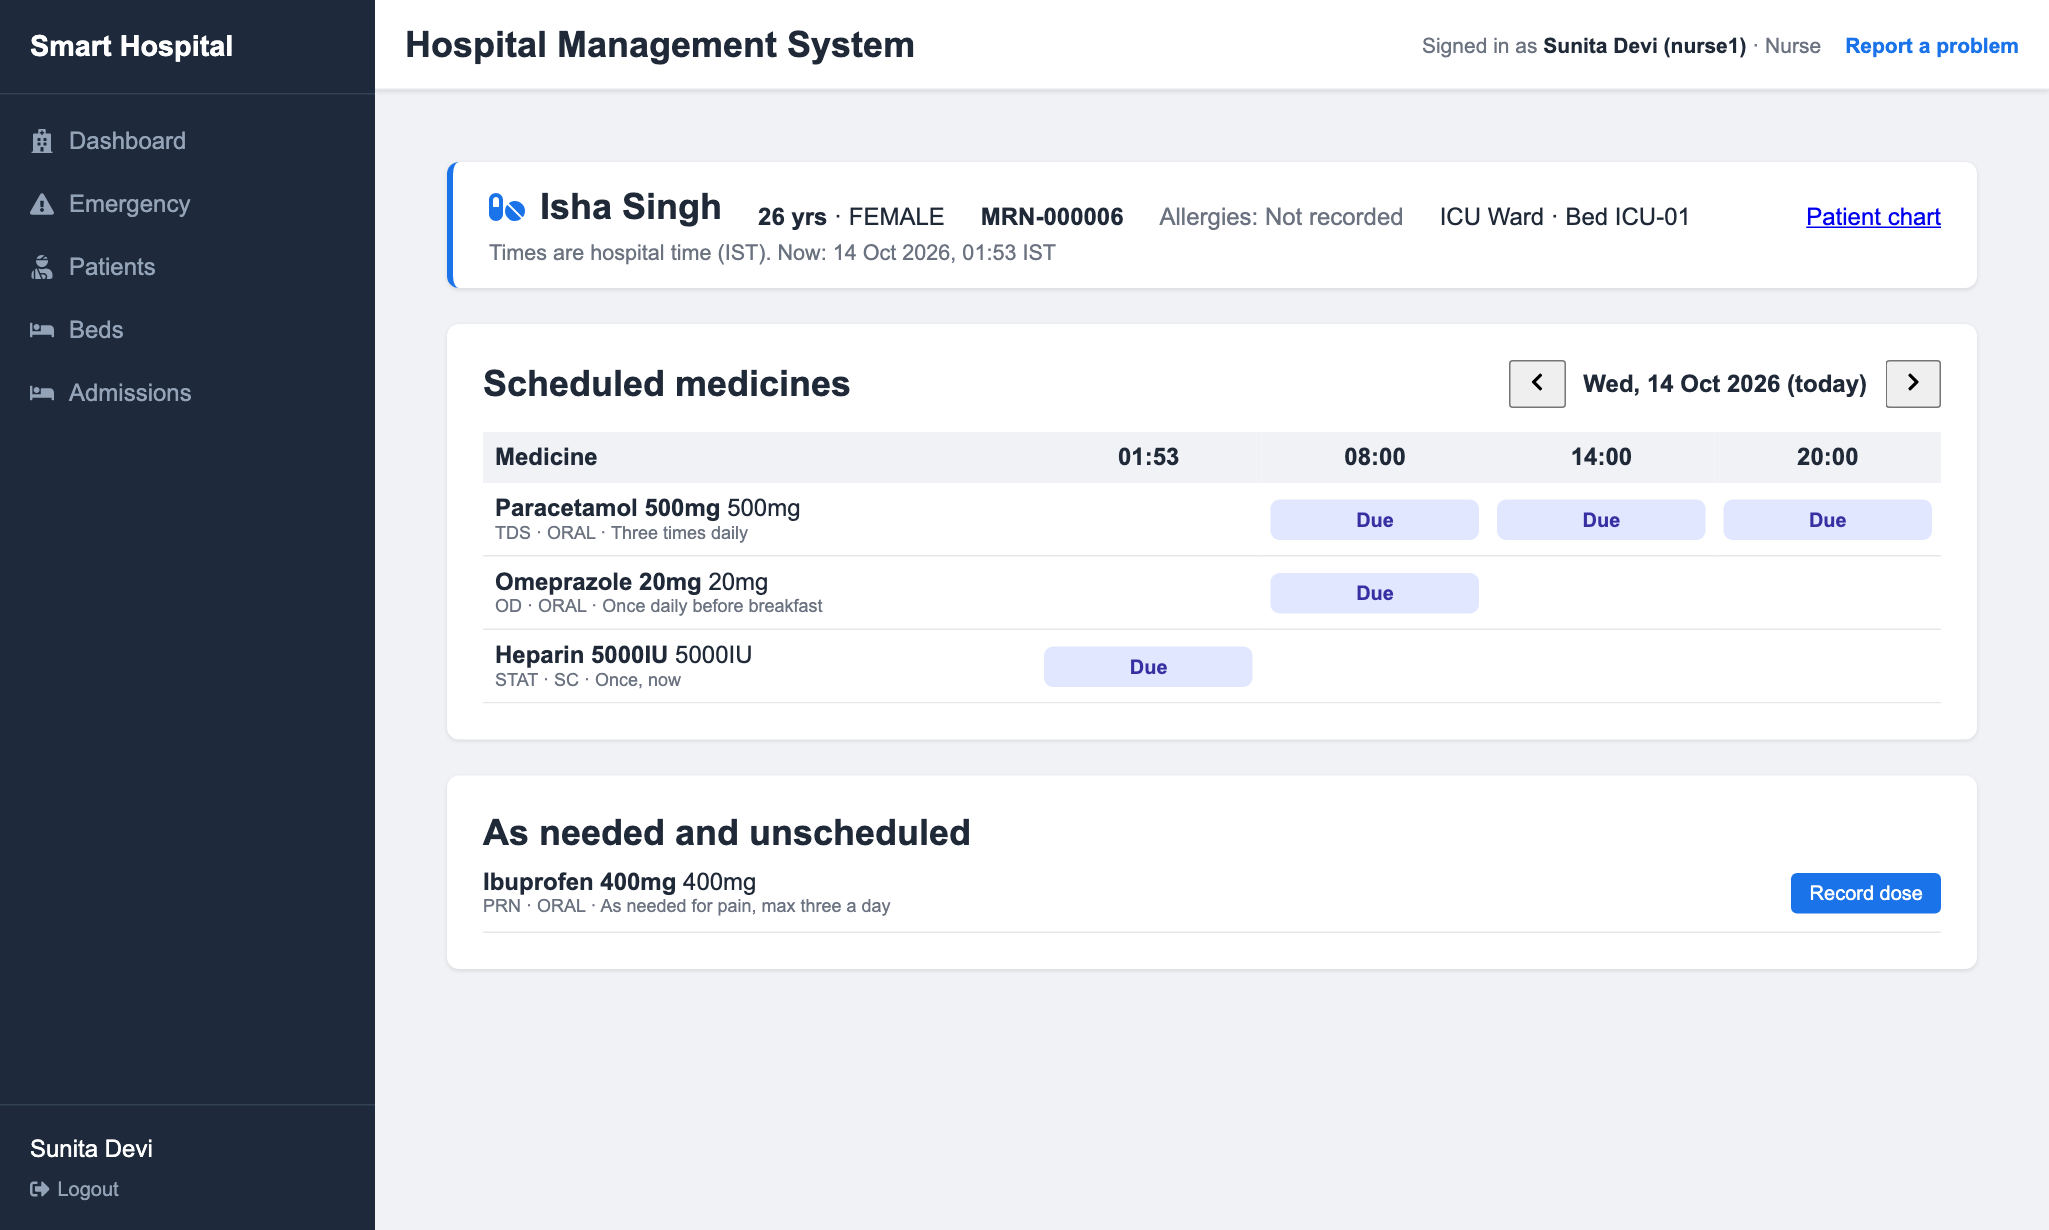
\includegraphics[width=0.485\textwidth]{nurse-mar.png} & 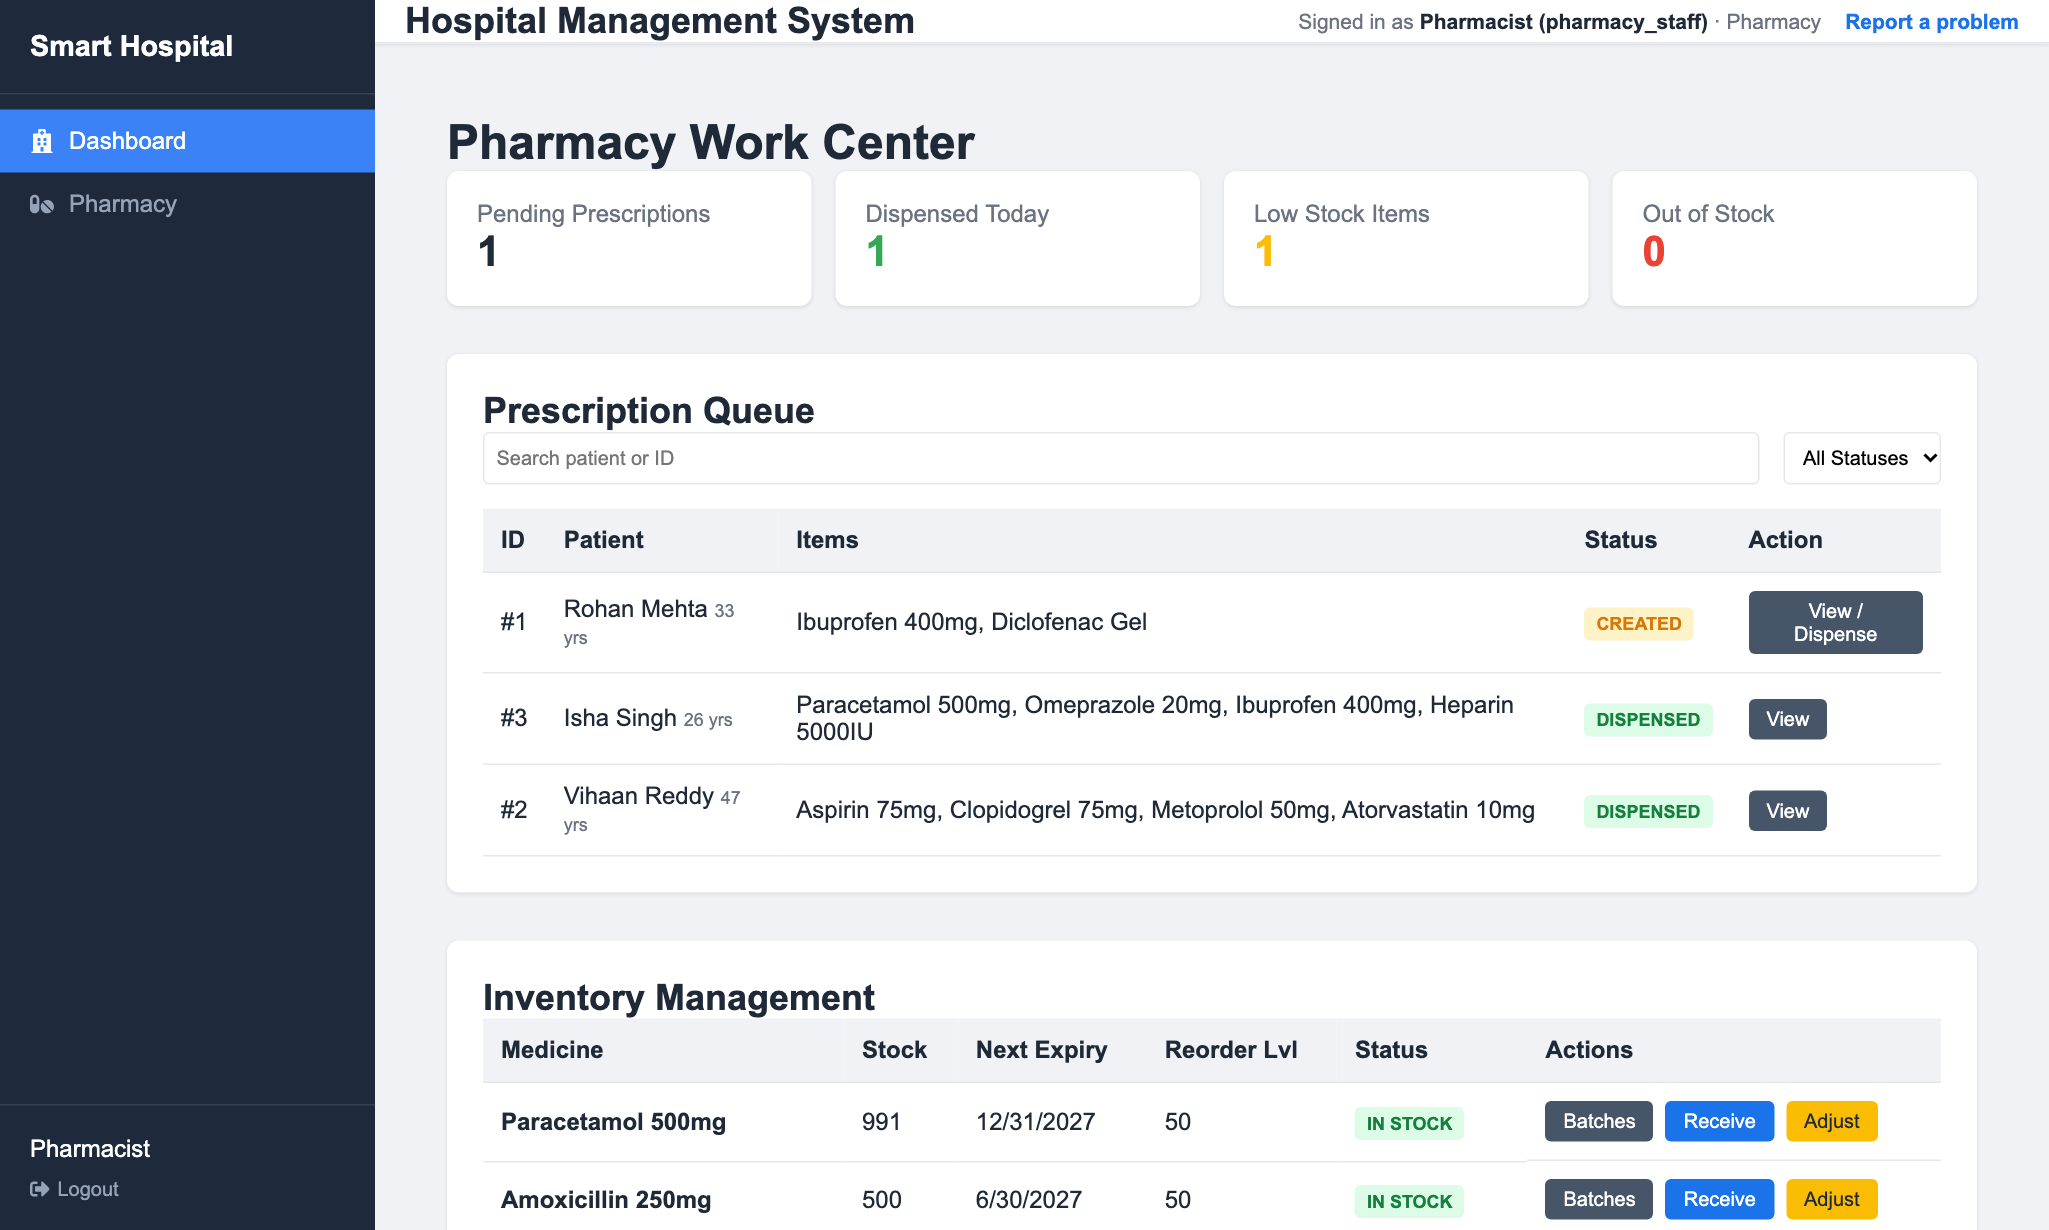
\includegraphics[width=0.485\textwidth]{pharmacy-dashboard.png} \\
\small (c) Nurse: medication administration record & \small (d) Pharmacy: dispense queue and stock \\
\end{tabular}
\caption{Major screens, one per role (test data)}\label{fig:screens}
\end{figure}

\section{Database Operations through the Application}
Each screen action becomes SQL in one transaction, and the result is visible in MySQL. The patient-journey browser
test drives these screens and then checks the rows in the database.

{\small
\begin{tabularx}{\textwidth}{@{}R{4.6cm}Y@{}}
\toprule
\textbf{Action on screen} & \textbf{Statements on hospital\_db} \\\midrule
Register a patient (reception) & \tbl{INSERT INTO patients}; \tbl{INSERT INTO audit\_logs} (CREATE\_PATIENT) \\
Book an appointment & \tbl{INSERT INTO appointments} (a duplicate slot fails the UNIQUE key: 409 ``Double booking detected'') \\
Mark arrived, start, finish a visit & \tbl{SELECT \dots{} FOR UPDATE} on the appointment and encounter; \tbl{INSERT}/\tbl{UPDATE encounters}; \tbl{UPDATE appointments SET status} \\
Record vital signs (nurse) & \tbl{INSERT INTO vital\_signs} (refused by the CHECKs if out of range) \\
Dispense (pharmacy) & Listing in Section~8.7: locks, \tbl{UPDATE} items and batches, \tbl{INSERT} movements \\
Admit, discharge (doctor) & \tbl{INSERT INTO admissions} / \tbl{UPDATE admissions SET status = 'DISCHARGED'}; triggers update the bed, the workload and \tbl{bed\_assignment\_log} \\
Edit a patient's details & \tbl{UPDATE patients}; the audit row names the changed fields, never their values \\
Cancel a prescription & \tbl{UPDATE prescriptions SET status = 'CANCELLED'}; pending doses \tbl{UPDATE medication\_administrations SET status = 'CANCELLED'} \\
Assign a nurse to a ward (admin) & \tbl{SELECT \dots{} FOR UPDATE} on the nurse's account, then on any assignment sharing a day (409 if one exists); \tbl{INSERT INTO nurse\_ward\_assignments} \\
End an assignment & \tbl{UPDATE nurse\_ward\_assignments SET end\_date = ?, ended\_at = ?}: the nurse loses the ward at once \\
Cancel an assignment not yet started & \tbl{DELETE FROM nurse\_ward\_assignments}, refused (409) once it has started \\
\bottomrule
\end{tabularx}}
Clinical records are not deleted through the application: they are kept, and corrections are recorded as new
states (for example a visit marked ENTERED\_IN\_ERROR), which the audit log requires. The one delete is cancelling a
nurse assignment before its first day, which never gave access to anything; the audit log keeps its dates.
